\documentclass[11pt]{article}

\usepackage{amsmath, amssymb}
\usepackage{physics}
\usepackage{geometry}
\usepackage{graphicx}
\usepackage{siunitx}
\usepackage{setspace}
\usepackage{tcolorbox}
\usepackage{tikz}
\usetikzlibrary{arrows.meta}

\geometry{margin=1in}
\setstretch{1.15}

\title{\textbf{Continuity, Bernoulli's Equation, and Hydrostatics}}
\author{}
\date{}

\begin{document}
\maketitle

%------------------------------------------------
\section{Hydrostatic Pressure and the U-Tube}

For a fluid at rest, pressure varies with depth according to
\begin{equation}
    P = P_0 + \rho g h ,
\end{equation}
where $P_0$ is the surface pressure and $h$ is the depth below the surface.

\subsection*{U-Tube with Two Fluids}

At equilibrium, pressures at the same horizontal level must be equal:
\begin{align}
    P_0 + \rho_{\text{oil}} g h_{\text{oil}}
    &=
    P_0 + \rho_{\text{water}} g h_{\text{water}} .
\end{align}

Canceling $P_0$,
\begin{equation}
    \boxed{
    \rho_{\text{oil}} h_{\text{oil}}
    =
    \rho_{\text{water}} h_{\text{water}}
    }
\end{equation}

\begin{tcolorbox}
\textbf{Key Idea:}  
In static fluids, pressure depends only on depth and density.
\end{tcolorbox}

\subsection*{Example: U-Shaped Tube with Oil and Water}

A U-shaped tube is open to the atmosphere on both sides. One side contains oil
($\rho_{\text{oil}} = 0.5\,\text{g/cm}^3$), and the other contains water
($\rho_{\text{water}} = 1.0\,\text{g/cm}^3$).

If the oil column has height $h_{\text{oil}} = 20\,\text{cm}$, find the height
$h_{\text{water}}$ of the water column.

\paragraph{Solution}

At the same horizontal level, pressures are equal:
\[
\rho_{\text{oil}} g h_{\text{oil}} = \rho_{\text{water}} g h_{\text{water}}.
\]

Thus,
\[
h_{\text{water}}
= \frac{\rho_{\text{oil}}}{\rho_{\text{water}}} h_{\text{oil}}
= \frac{0.5}{1.0}(20\,\text{cm})
= 10\,\text{cm}.
\]




%------------------------------------------------
\section{Continuity Equation}

\subsection*{Mass Conservation}

For steady flow, mass is conserved:
\begin{equation}
    \boxed{
    \frac{\Delta m_{\text{in}}}{\Delta t}
    =
    \frac{\Delta m_{\text{out}}}{\Delta t}
    }
\end{equation}

Using $\Delta m = \rho \Delta V$,
\begin{equation}
    \rho \frac{\Delta V_{\text{in}}}{\Delta t}
    =
    \rho \frac{\Delta V_{\text{out}}}{\Delta t}.
\end{equation}

Since $\Delta V = A \Delta x$ and $v = \Delta x / \Delta t$,
\begin{equation}
    \rho A_{\text{in}} v_{\text{in}}
    =
    \rho A_{\text{out}} v_{\text{out}}.
\end{equation}

For an incompressible fluid ($\rho =$ constant),
\begin{equation}
    \boxed{
    A_{\text{in}} v_{\text{in}} = A_{\text{out}} v_{\text{out}}
    }
\end{equation}

\begin{tcolorbox}
\textbf{Consequence:}  
If a pipe narrows, the fluid speed increases.
\end{tcolorbox}

%------------------------------------------------
\begin{figure}[h]
\centering
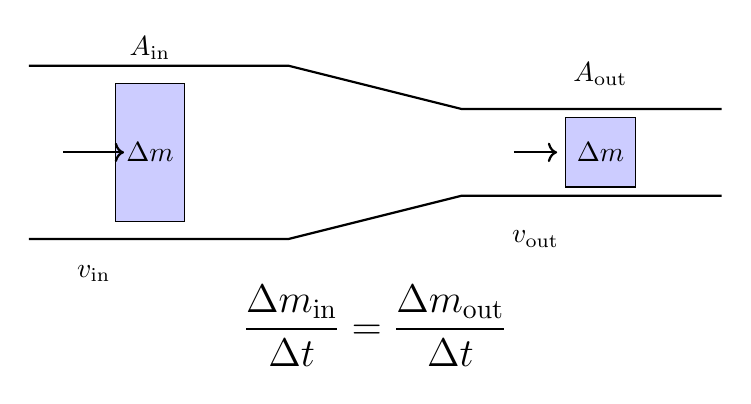
\begin{tikzpicture}[scale=1.1]

% Pipe walls
\draw[thick] (-4,1) -- (-1,1) -- (1,0.5) -- (4,0.5);
\draw[thick] (-4,-1) -- (-1,-1) -- (1,-0.5) -- (4,-0.5);

% Fluid elements
\draw[fill=blue!20] (-3,0.8) rectangle (-2.2,-0.8);
\draw[fill=blue!20] (2.2,0.4) rectangle (3,-0.4);

% Velocity arrows
\draw[->, thick] (-3.6,0) -- (-2.9,0);
\draw[->, thick] (1.6,0) -- (2.1,0);

% Labels
\node at (-2.6,1.2) {$A_{\text{in}}$};
\node at (2.6,0.9) {$A_{\text{out}}$};

\node at (-3.25,-1.4) {$v_{\text{in}}$};
\node at (1.85,-1.0) {$v_{\text{out}}$};

\node at (-2.6,0) {$\Delta m$};
\node at (2.6,0) {$\Delta m$};

\node at (0,-2) {\Large $\displaystyle
\frac{\Delta m_{\text{in}}}{\Delta t}
=
\frac{\Delta m_{\text{out}}}{\Delta t}
$};

\end{tikzpicture}
\caption{Mass conservation for steady incompressible flow. The same mass of fluid enters and exits the pipe in equal time intervals, even though the speed changes.}
\end{figure}

\subsection*{Example: Filling a Bucket}

A hose fills a $10\,\text{L}$ bucket in $20\,\text{s}$.  
The hose opening has cross-sectional area $A = 10\,\text{cm}^2$.

Find the speed of the water exiting the hose.

\paragraph{Solution}

Convert volume:
\[
10\,\text{L} = 10 \times 10^{-3}\,\text{m}^3.
\]

Volume flow rate:
\[
Q = \frac{\Delta V}{\Delta t}
= \frac{10 \times 10^{-3}}{20}
= 5 \times 10^{-4}\,\text{m}^3/\text{s}.
\]

Using $Q = Av$:
\[
v = \frac{Q}{A}
= \frac{5 \times 10^{-4}}{10 \times 10^{-4}}
= 0.5\,\text{m/s}.
\]




%------------------------------------------------
\section{Bernoulli's Equation}

Work done by pressure forces on a fluid element:
\begin{equation}
    W = P_1 \Delta V - P_2 \Delta V.
\end{equation}

Change in kinetic energy:
\begin{equation}
    \Delta K = \frac{1}{2} \rho \Delta V (v_2^2 - v_1^2).
\end{equation}

Change in gravitational potential energy:
\begin{equation}
    \Delta U = \rho \Delta V g (y_2 - y_1).
\end{equation}

Using $W = \Delta K + \Delta U$ and dividing by $\Delta V$:
\begin{equation}
    \boxed{
    P + \frac{1}{2}\rho v^2 + \rho g y = \text{constant}
    }
\end{equation}

%------------------------------------------------
\section*{Assumptions}

\begin{itemize}
    \item Steady flow
    \item Incompressible fluid
    \item Negligible viscosity
    \item Flow along a streamline
\end{itemize}

\subsection*{Example: Bernoulli Without Gravity}

Water flows horizontally through a pipe that narrows from
$A_1 = 4\,\text{cm}^2$ to $A_2 = 1\,\text{cm}^2$.
The speed at the wide section is $v_1 = 1\,\text{m/s}$.

Find the pressure difference $P_1 - P_2$.

\paragraph{Solution}

From continuity:
\[
v_2 = \frac{A_1}{A_2} v_1 = 4\,\text{m/s}.
\]

Bernoulli (same height):
\[
P_1 - P_2 = \frac{1}{2}\rho (v_2^2 - v_1^2).
\]

Using $\rho = 1000\,\text{kg/m}^3$:
\[
P_1 - P_2 = \frac{1}{2}(1000)(16 - 1)
= 7500\,\text{Pa}.
\]

\begin{figure}[h]
\centering
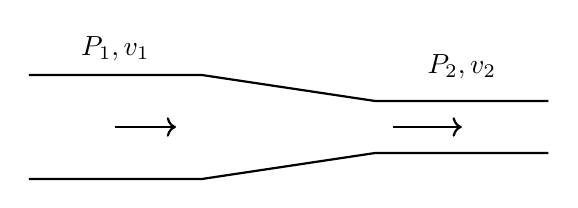
\begin{tikzpicture}[scale=1.1]

% Pipe
\draw[thick] (-3,0.6) -- (-1,0.6) -- (1,0.3) -- (3,0.3);
\draw[thick] (-3,-0.6) -- (-1,-0.6) -- (1,-0.3) -- (3,-0.3);

% Arrows
\draw[->, thick] (-2,0) -- (-1.3,0);
\draw[->, thick] (1.2,0) -- (2,0);

% Labels
\node at (-2,0.9) {$P_1, v_1$};
\node at (2,0.7) {$P_2, v_2$};

\end{tikzpicture}
\caption{Horizontal flow: pressure decreases as speed increases.}
\end{figure}

\subsection*{Example: Bernoulli With Gravity}

Water flows upward in a pipe from point 1 to point 2.
The speed is the same at both points.
Point 2 is $5\,\text{m}$ higher than point 1.

Find the pressure difference $P_1 - P_2$.

\paragraph{Solution}

Since $v_1 = v_2$, kinetic terms cancel:
\[
P_1 - P_2 = \rho g (y_2 - y_1).
\]

Using $\rho = 1000\,\text{kg/m}^3$:
\[
P_1 - P_2 = (1000)(9.8)(5) = 4.9 \times 10^4\,\text{Pa}.
\]

\begin{figure}[h]
\centering
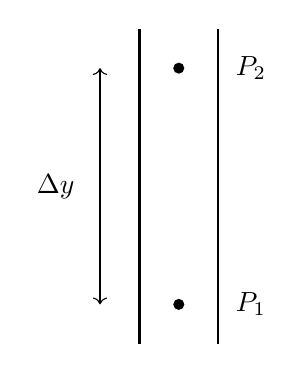
\begin{tikzpicture}[scale=1]

% Vertical pipe
\draw[thick] (0,-2) -- (0,2);
\draw[thick] (1,-2) -- (1,2);

% Points
\fill (0.5,-1.5) circle (2pt);
\fill (0.5,1.5) circle (2pt);

% Labels
\node[right] at (1.1,-1.5) {$P_1$};
\node[right] at (1.1,1.5) {$P_2$};

\draw[<->] (-0.5,-1.5) -- (-0.5,1.5);
\node[left] at (-0.7,0) {$\Delta y$};

\end{tikzpicture}
\caption{Pressure decreases with height in steady flow.}
\end{figure}


\subsection*{Example: Bernoulli With Gravity \emph{and} Area Change}

Water flows steadily upward through a pipe that both \textbf{narrows} and \textbf{rises}.
At point 1 (lower, wide section): $A_1 = 4\,\text{cm}^2$, $v_1 = 2.0\,\text{m/s}$, $y_1 = 0$.
At point 2 (higher, narrow section): $A_2 = 1\,\text{cm}^2$, $y_2 = 3.0\,\text{m}$.

Assume incompressible, nonviscous flow. Find $P_1 - P_2$.

\paragraph{Solution}

\textbf{Step 1: Continuity to get $v_2$.}
\[
A_1 v_1 = A_2 v_2
\quad \Rightarrow \quad
v_2 = \frac{A_1}{A_2}v_1 = 4(2.0)=8.0\,\text{m/s}.
\]

\textbf{Step 2: Bernoulli between 1 and 2.}
\[
P_1 + \frac12\rho v_1^2 + \rho g y_1
=
P_2 + \frac12\rho v_2^2 + \rho g y_2
\]
so
\[
P_1 - P_2 = \frac12\rho\left(v_2^2 - v_1^2\right) + \rho g (y_2-y_1).
\]

With $\rho = 1000\,\text{kg/m}^3$ and $g=9.8\,\text{m/s}^2$:
\[
P_1 - P_2
=
\frac12(1000)\left(8.0^2-2.0^2\right)
+(1000)(9.8)(3.0)
\]
\[
=
500(64-4) + 29400
=
500(60)+29400
=
30000+29400
=
5.94\times 10^4\,\text{Pa}.
\]

\[
\boxed{P_1 - P_2 \approx 5.9\times 10^4\ \text{Pa}}
\]

\vspace{5cm}

Flow rises and narrows: speed increases (continuity) and pressure drops further due to both higher speed and higher elevation (Bernoulli).


\end{document}
